% !TEX root = FDS_Technical_Reference_Guide.tex

\chapter{Overview of the FDS Model}

\label{basisformodel}

This chapter presents the governing equations of FDS and an outline of the general solution procedure. Details are included in subsequent chapters. The purpose of this chapter is to highlight aspects of the solution methodology that make it practical for thermally-driven flow simulations, in particular fire. Some of the major features of the model, in its default operation, are:
\begin{itemize}
\item Low Mach, large-eddy simulation (LES)
\item Explicit, second-order, kinetic-energy-conserving numerics
\item Structured, uniform, staggered grid
\item Simple immersed boundary method for treatment of flow obstructions
\item Generalized ``lumped species'' method (simplified chemistry using a reaction progress variable)
\item Deardorff eddy viscosity subgrid closure
\item Constant turbulent Schmidt and Prandtl numbers
\item Eddy dissipation concept (fast chemistry) for single-step reaction between fuel and oxidizer
\item Gray gas radiation with finite volume solution to the radiation transport equation
\end{itemize}
The model, however, is not limited to these simple algorithms. For example, the user may specify multiple reactions, finite-rate chemistry, a wide-band radiation model, and a variety of other special features. The more detailed physics incur increased computational cost, and it is incumbent on the user to justify the added expense in terms of improved accuracy for a particular application.  The default model options have been selected based on results from a wide variety of full-scale validation experiments \cite{FDS_Validation_Guide}.

The algorithm outlined below has evolved over roughly three decades. Initially, it was designed to study buoyant plumes in the Boussinesq limit; that is, the fluid was assumed incompressible but included a source term for buoyancy. This approach was based on a long tradition in fire research of modeling smoke movement using dyed salt water introduced into a tank filled with fresh water. Eventually, this approach proved too limiting, but some of the major features of the algorithm, like the low Mach number approximation, were retained.

\section{LES Formalism}
\label{filteredfields}

The equations for large-eddy simulation (LES) are derived by applying a low-pass filter, parameterized by a width $\Delta$, to the transport equations for mass, momentum and energy.  For our purposes, it is sufficient to think of the filtered fields in the LES equations as cell means.  For example, in 1D the filtered density for a cell of width $\Delta$ is
\begin{equation}
\label{eqn_filtered_density}
\bar{\rho}(x,t) = \frac{1}{\Delta}\int_{x-\Delta/2}^{x+\Delta/2} \rho(r,t) \d r \mbox{.}
\end{equation}
In FDS, the filter width $\Delta$ is equivalent to the local cell size $\delta x$ and is a key parameter in the submodels for the turbulent viscosity and the reaction time scale discussed later.  The practice of taking $\Delta = \delta x$ is called implicit filtering.  It is important to appreciate, however, that implicit filtering does not imply dissipative numerics.  FDS employs kinetic-energy-conserving central difference schemes for momentum with physically-based closures for the turbulent stress.  In what follows, the filter formalism is relaxed (the overline notation is suppressed for clarity) since no explicit filtering operations are performed in the algorithm.  A detailed derivation of the formal LES equations is presented in Chapter \ref{momentum_chapter}.

\section{Numerical Grid}
\label{govequations}

Because FDS was designed to simulate thermally-driven flows within buildings, the most obvious and simplest numerical grid is rectilinear. In fact, because FDS is a large eddy simulation (LES) model, uniform meshing is preferred, and the only numerical parameters chosen by the end user are the three dimensions of the grid. Once established, it is relatively simple to define rectangular obstructions that define the geometry to the level of resolution determined by the grid. These obstructions ``snap'' to the underlying grid, a very elementary form of an immersed boundary method (IBM). Unstructured geometry is possible in FDS by virtue of a cutcell method as described in Sec.~\ref{sec:unstructured_geometry}.

\subsection{The Staggered Grid}
\label{sec:staggered_grid}

The governing equations are approximated using second-order accurate finite differences on a collection of uniformly spaced three-dimensional grids. Multiple meshes can be processed in parallel using Message Passing Interface (MPI) libraries. Scalar quantities are assigned to the center of each grid cell; the velocity components at the appropriate cell faces; and vorticity components at cell edges. This is what is commonly referred to as a staggered grid \cite{Harlow:1,Morinishi}.  Its main purpose is to avoid ``checker-boarding'' in pressure-velocity coupling by naturally representing the pressure cell velocity divergence, a very important thermodynamic quantity in the model. Figure~\ref{variable_positions} displays where in a given grid cell the various flow variables are located.

\begin{figure}[!h]
\centering
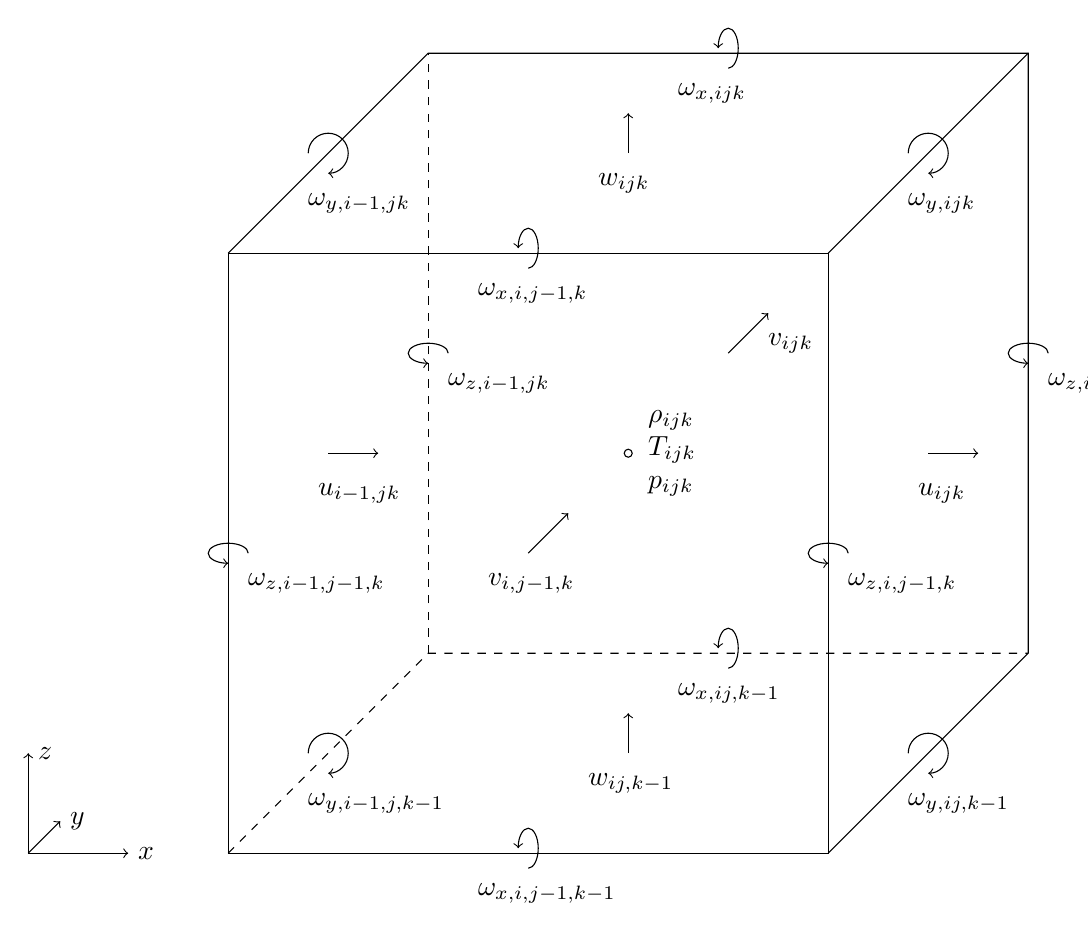
\begin{tikzpicture}[x=1in,y=1in]
\draw [->] (-1,0) -- (-0.5,0); \node[text width=1, anchor=west] at (-0.5,0) {$x$};
\draw [->] (-1,0) -- (-0.84,0.16); \node[text width=1, anchor=west] at (-0.84,0.16) {$y$};
\draw [->] (-1,0) -- (-1,0.5); \node[text width=1, anchor=west] at (-1,0.5) {$z$};
\draw (0,0) rectangle (3,3);
\draw (2,2) circle (0.02); \node[text width=1, anchor=west] at (2.05,2.0) {$\rho_{ijk}$ \\ $T_{ijk}$ \\ $p_{ijk}$ };
\draw (0,0) (3,0) -- (4,1) -- (4,4) -- (1,4) -- (0,3);
\draw (0,0) (3,3) -- (4,4);
\draw [dashed] (0,0) (0,0) -- (1,1) -- (4,1);
\draw [dashed] (0,0) (1,1) -- (1,4);
\draw [->] (0.5,2) -- (0.75,2); \node[text width=1, anchor=west] at (0.4,1.8) {$u_{i-1,jk}$};
\draw [->] (3.5,2) -- (3.75,2); \node[text width=1, anchor=west] at (3.4,1.8) {$u_{ijk}$};
\draw [->] (1.5,1.5) -- (1.7,1.7); \node[text width=1, anchor=west] at (1.25,1.35) {$v_{i,j-1,k}$};
\draw [->] (2.5,2.5) -- (2.7,2.7); \node[text width=1, anchor=west] at (2.65,2.55) {$v_{ijk}$};
\draw [->] (2.0,0.5) -- (2.0,0.7); \node[text width=1, anchor=west] at (1.75,0.35) {$w_{ij,k-1}$};
\draw [->] (2.0,3.5) -- (2.0,3.7); \node[text width=1, anchor=west] at (1.80,3.35) {$w_{ijk}$};
\draw [->] (0.4,3.5) arc (180:-90:.1); \node[text width=1, anchor=west] at (0.35,3.25) {$\omega_{y,i-1,jk}$};
\draw [->] (3.4,3.5) arc (180:-90:.1); \node[text width=1, anchor=west] at (3.35,3.25) {$\omega_{y,ijk}$};
\draw [->] (0.4,0.5) arc (180:-90:.1); \node[text width=1, anchor=west] at (0.35,0.25) {$\omega_{y,i-1,j,k-1}$};
\draw [->] (3.4,0.5) arc (180:-90:.1); \node[text width=1, anchor=west] at (3.35,0.25) {$\omega_{y,ij,k-1}$};
\draw [->] (1.5,-0.075) arc (-90:180:0.05 and 0.1); \node[text width=1, anchor=west] at (1.2,-0.2) {$\omega_{x,i,j-1,k-1}$};
\draw [->] (1.5, 2.925) arc (-90:180:0.05 and 0.1); \node[text width=1, anchor=west] at (1.2, 2.8) {$\omega_{x,i,j-1,k}$};
\draw [->] (2.5, 0.925) arc (-90:180:0.05 and 0.1); \node[text width=1, anchor=west] at (2.2, 0.8) {$\omega_{x,ij,k-1}$};
\draw [->] (2.5, 3.925) arc (-90:180:0.05 and 0.1); \node[text width=1, anchor=west] at (2.2, 3.8) {$\omega_{x,ijk}$};
\draw [->] (0.1, 1.5) arc (0:270:0.1 and 0.05); \node[text width=1, anchor=west] at (0.05, 1.35) {$\omega_{z,i-1,j-1,k}$};
\draw [->] (3.1, 1.5) arc (0:270:0.1 and 0.05); \node[text width=1, anchor=west] at (3.05, 1.35) {$\omega_{z,i,j-1,k}$};
\draw [->] (1.1, 2.5) arc (0:270:0.1 and 0.05); \node[text width=1, anchor=west] at (1.05, 2.35) {$\omega_{z,i-1,jk}$};
\draw [->] (4.1, 2.5) arc (0:270:0.1 and 0.05); \node[text width=1, anchor=west] at (4.05, 2.35) {$\omega_{z,ijk}$};
\end{tikzpicture}
\caption[Position of flow variables in a grid cell]{Position of flow variables in grid cell $ijk$. The arrows indicate the positive direction of the given variable. Scalar variables, such as the density, $\rho$, temperature, $T$, and pressure, $p$, are defined at the cell center. Velocity components, $\mathbf{u}=(u,v,w)$, are defined at their respective cell faces, and vorticity components, $\vec{\omega}=(\omega_x,\omega_y,\omega_z)$, are located at cell edges.}
\label{variable_positions}
\end{figure}

\subsection{Cell Edges}
\label{sec:cell_edges}

In the FDS staggered grid arrangement, cell edges are the storage location of both off-diagonal stresses and vorticity.  The computational edge variable position environment is described below.

\begin{figure}[!h]
\centering
\scalebox{0.75}{
\begin{tikzpicture}[x=1in,y=1in]
\draw [->] (-1,2) -- (-0.5,2); \node[text width=1, anchor=west] at (-0.5,2) {$x$};
\draw [->] (-1,2) -- (-0.84,2.16); \node[text width=1, anchor=west] at (-0.84,2.16) {$y$};
\draw [->] (-1,2) -- (-1,2.5); \node[text width=1, anchor=west] at (-1,2.5) {$z$};

\draw (0,0) (-1,1) -- (0,2) -- (3,2) -- (2,1) -- (-1,1);

\draw [->] (1.0,1.5) -- (1.0,1.7); \node[text width=1, anchor=west] at (0.80,1.35) {$w_{ijk}$};
\draw [->] (2.0,2.5) -- (2.0,2.7); \node[text width=1, anchor=west] at (1.80,2.35) {$w_{i,j+1,k}$};

\draw [->] (1.4,0.4) -- (1.6,0.6); \node[text width=1, anchor=west] at (1.40,0.30) {$v_{ijk}$};
\draw [->] (1.4,3.4) -- (1.6,3.6); \node[text width=1, anchor=west] at (1.40,3.70) {$v_{i,j,k+1}$};

\draw [line width=1mm] (0,0) (0,2) -- (3,2); \node[text width=1, anchor=west] at (3.2, 2) {{\tt IEC}\;=\;1};

\draw [->] (1.5, 1.925) arc (-90:180:0.05 and 0.1); \node[text width=1, anchor=west] at (1.2, 1.8) {$\omega_{x,ijk}$};

\draw [dashed] (0,0) (0,2) -- (1,3) -- (3,3);
\draw (0,0) (3,3) -- (4,3) -- (3,2);

\draw (0,0) (0,2) -- (0,5) -- (3,5) -- (3,2) -- (0,2);

\draw (0,0) (0,1) -- (0,-1) -- (3,-1) -- (3,2);
\draw [dashed] (0,0) (0,1) -- (0,2);

\end{tikzpicture}
}
\caption[Position of flow variables around a computational edge]{Position of flow variables around a computational edge along the $x$ axis.  The Index of the Edge Component (\ct{IEC}) is 1 in this case.  The orientations of the faces (defined by the directions normal to the faces) that connect to the edge are \ct{IOR} = $\pm2$, $\pm3$.  The vorticity around the edge is $\omega_x = \partial w/\partial y - \partial v/\partial z$.}
\label{fig:edge_positions}
\end{figure}

\section{Mass and Species Transport}
\label{sec_lumped_species}

The most basic description of the chemistry of fire is a reaction of a hydrocarbon fuel with oxygen that produces carbon dioxide and water vapor. Because fire is a relatively inefficient combustion process involving multiple fuel gases that contain more than just carbon and hydrogen atoms, the number of gas species to keep track of in the simulation is almost limitless. However, to make the simulations tractable, we limit the number of fuels to one, usually, and the number of reactions to just one or two. We also leave open the possibility that the reaction may not proceed for lack of sufficient oxygen in the incoming air stream, as when a fire in a closed compartment extinguishes itself. Even with this simplified approach to the chemistry, we still need to track at least six gas species (Fuel, O$_2$, CO$_2$, H$_2$O, CO, N$_2$) plus soot particulate. If we assume a single-step reaction, we do not need to solve explicitly seven transport equations. In fact, we only need to solve two -- one for the fuel and one for the products. The air is everything that is neither fuel nor products. However, to ensure realizability of species mass fractions, our strategy is to solve a transport equation for each species mass density and then to obtain the mixture mass density by summation of the species densities.

Whereas the fuel is usually a single gas species, the air and products are what are often referred to as ``lumped species''. A lumped species represents a mixture of gas species that transport together (i.e., the lumped species has a single set of transport properties) and react together, and from the point of view of the numerical model, a lumped species can be treated as a single species. In fact, the mass transport equations make no distinction between a single or lumped species. For example, air is a lumped species that consists of nitrogen, oxygen, and trace amounts of water vapor and carbon dioxide. We use the symbols $Z_A$, $Z_F$, and $Z_P$ to denote the mass fractions of air, fuel and products.  The lumped species mass fractions are linearly related to the primitive species mass fractions, $Y_\alpha$; thus, conversion from one to the other is a simple matter of performing a matrix multiplication.  For example, the complete combustion of methane:
\be \mathrm{CH_4 + 2 \, \left( O_2 + 3.76 \, N_2 \right)  \rightarrow CO_2 +2 \, H_2O + 7.52 \, N_2} \ee
is expressed as
\be \hbox{Fuel} + 2 \, \hbox{Air} \rightarrow \hbox{Products} \ee
and the primitive species can be recovered from the lumped species via
\be \left[ \begin{array} {c c c}
0.77 & 0.00 & 0.73 \\
0.23 & 0.00 & 0.00 \\
0.00 & 1.00 & 0.00 \\
0.00 & 0.00 & 0.15 \\
0.00 & 0.00 & 0.12  \end{array}
\right]
\left[ \begin{array} {c} Z_{\rm A} \\ Z_{\rm F} \\ Z_{\rm P} \end{array} \right] =
\left[ \begin{array} {c} Y_\NTWO \\ Y_\OTWO \\ Y_{\scriptscriptstyle \mathrm{CH_4}} \\ Y_\COTWO \\ Y_{\scriptscriptstyle \mathrm{H_2O}} \end{array} \right]
 \ee
Notice that the columns of the matrix are the mass fractions of the primitive species within a given lumped species.

The transport equation for each of the lumped species has the same form as the transport equation for a single species:
\be \dod{ }{t}(\rho Z_\alpha) + \nabla\!\cdot (\rho Z_\alpha \bu) = \nabla\!\cdot (\rho D_\alpha \nabla Z_\alpha) + \dm_\alpha''' + \dm_{\rm b,\alpha}''' \label{species} \ee
Note that the source term on the right hand side represents the addition of mass from evaporating droplets or other subgrid-scale
particles that represent sprinkler and fuel sprays, vegetation, and any other type of small, unresolvable object. These
objects are assumed to occupy no volume; thus, they are seen by the governing equations as point sources of mass, momentum, and energy. It is important to
note, however, that the evaporated mass species must be one for which an explicit transport equation is solved. For example, water vapor is a product of
combustion, but it is also formed by evaporating sprinkler droplets. In cases such as these, there needs to be an explicit transport equation for water
vapor to distinguish between that which is formed by combustion and that which is evaporated from the droplets. Here $\dm_{\rm b,\alpha}'''$ is the production rate of species $\alpha$ by evaporating droplets or particles.

The mass density is obtained from $\rho = \sum (\rho Z)_\alpha$.  The summation of Eq.~(\ref{species}) over all $N_s$ species gives
\be \dod{\rho}{t} + \nabla\!\cdot (\rho \bu)  =  \dm_{\rm b}'''  \label{mass} \ee
because $\sum Z_\alpha=1$ and $\sum \dm_\alpha''' = 0$ and $\sum \dm_{\rm b,\alpha}'''=\dm_{\rm b}'''$, by definition, and because it is assumed that $\sum \rho D_\alpha \nabla Z_\alpha = 0$. This last assertion is not true, in general.  The diffusive flux for the most abundant local species is corrected to enforce the constraint.




\paragraph{Enforcing Realizability} ~\\

\noindent Realizability of species mass fractions requires $Y_\alpha \ge 0$ for all $\alpha$ and $\sum Y_\alpha = 1$.  Note that this is more restrictive than the boundedness constraint, which simply requires $0 \le Y_\alpha \le 1$.

If $(\rho Y)_\alpha$ obeys boundedness, $(\rho Y)_\alpha \ge 0$, and we solve $N_s$ species equations obtaining the density via $\rho = \sum_{\alpha=1}^{N_s} (\rho Y)_\alpha$, then mass fractions obtained by $Y_\alpha = (\rho Y)_\alpha/\rho$ are \emph{guaranteed to be realizable} (for $\rho>0$).  Thus, we have reduced the realizability problem to the ``easier'' problem of boundedness for $(\rho Y)_\alpha$. Details of the scalar boundedness correction are discussed in Appendix \ref{app_boundedness}.

With this approach we must take care to ensure $\sum \rho D_\alpha \nabla Z_\alpha = 0$.  Our strategy is to absorb any errors in diffusive transport into the most abundant species \emph{locally}.  That is, for a given cell face we set $\rho D_m \nabla Z_m = -\sum_{\alpha\ne m} \rho D_\alpha \nabla Z_\alpha$, where $m$ is the most abundant species adjacent to that face.  Note that since FDS is typically used as an LES code mass transport by molecular diffusion may be two or three orders of magnitude less than turbulent transport, which uses the same turbulent diffusion coefficient for all species. Therefore, the errors in summation of the diffusive fluxes tend to be small.

\section{Low Mach Number Approximation}

For low speed applications like fire, Rehm and Baum~\cite{Rehm:1} observed that the spatially and temporally resolved pressure, $p$, can be decomposed into a ``background'' pressure, $\bp(z,t)$, plus a perturbation, $\tp(x,y,z,t)$, with only the background pressure retained in the equation of state (ideal gas law):
\be \bp = \rho T \R \sum_\alpha  \frac{Z_\alpha}{W_\alpha} \equiv \frac{\rho \R T}{\bW}  \label{basicstate1} \ee
Note that $z$ is the spatial coordinate in the direction of gravity; thus, the stratification of the atmosphere is included in the background pressure. The perturbation, $\tp$, drives the fluid motion. This approximation has a number of consequences. First, building compartments connected via a heating, ventilation, and air conditioning (HVAC) system can each maintain individual background pressures. The air flows between compartments can be
described in terms of the differences in the background pressures, eliminating the need to solve detailed flow equations within the ventilation ducts.

The second consequence of the low Mach number approximation is that the internal energy, $e$, and enthalpy, $h$, may be related in terms of the thermodynamic (background) pressure: $h = e + \bp/\rho$.  The energy conservation equation may then be written in terms of the {\em sensible enthalpy}, $h_{\rm s}$:
\be \dod{ }{t}(\rho h_{\rm s}) + \nabla\!\cdot (\rho h_{\rm s} \bu) = \DoD{\bp}{t} + \dq''' + \dq_{\rm b}''' - \nabla\!\cdot \dbq'' \label{energy} 
\ee
The term $\dq'''$ is the heat release rate per unit volume from a chemical reaction. The term $\dq_{\rm b}'''$ is the energy transferred to subgrid-scale droplets and particles. The term $\dbq''$ represents the conductive, diffusive, and radiative heat fluxes:
\be
   \dbq'' = -k \nabla T - \sum_\alpha h_{\rm s,\alpha} \, \rho \, D_\alpha \nabla Z_\alpha + \dbq_{\rm r}''  \label{bqdot_def}
\ee
where $k$ is the thermal conductivity , $D_\alpha$ is the diffusivity of species $\alpha$, and $\dbq_{\rm r}''$ is the radiative flux.

Eq.~(\ref{energy}) is not solved explicitly. Instead, the velocity divergence is factored out as follows:
\be
\label{eqn_simplediv1}
\Div\mathbf{u} = \frac{1}{\rho h_{\rm s}} \left[ \DoD{}{t} (\bp-\rho h_{\rm s}) + \dq''' + \dq_{\rm b}^\ppp - \Div \dot{\mathbf{q}}^\pp \right]
\ee
The hydrodynamics solver guarantees that Eq.~(\ref{eqn_simplediv1}) is satisfied.  It follows that Eq.~(\ref{energy}) is also satisfied (energy is conserved).

Expanding the material derivatives on the right hand side of Eq.~(\ref{eqn_simplediv1}) produces a fairly complicated expression for
the divergence that includes the source and diffusion terms from the mass, species, and energy conservation equations. Its importance to the overall algorithm is that it can be computed using only the thermodynamic variables $\rho$, $Z_\alpha$, and $\bp$. As will be shown below, the way to advance the flow velocity in time is to first estimate the thermodynamic variables at the next time step, compute the divergence, and then solve an equation for the pressure that will guarantee that the divergence of the updated velocity is identical to that computed solely from the thermodynamic variables.



\section{Momentum Transport}

Noting the vector identity $(\bu \cdot \nabla) \bu = \nabla|\bu|^2/2 - \bu\times\bo $, and defining the stagnation energy per unit mass, $\cH \equiv |\bu|^2/2 + \tp/\rho$, the momentum equation can be written (see Chapter \ref{momentum_chapter} for a detailed derivation)
\be
   \dod{\bu}{t} - \bu\times\bo + \nabla \cH - \tp \, \nabla \left( 1/\rho\right) = \frac{1}{\rho} \Big[ (\rho-\rho_0) \bg + \bof_{\rm b} + \nabla\!\cdot \btau \Big] \label{momeqnoncon}
\ee
The term $\bof_\text{b}$ represents the drag force exerted by the subgrid-scale particles and droplets. The viscous stress, $\btau$, is closed via gradient diffusion with the turbulent viscosity obtained from the Deardorff eddy viscosity model \cite{Deardorff:1980,Pope:2000}. It is convenient to write Eq.~(\ref{momeqnoncon}) in the form:
\be
   \dod{\bu}{t} + \bF + \nabla \cH  = 0
\ee
so that a Poisson equation for the pressure can be derived by taking its divergence:
\be
   \nabla^2 \cH = - \left[ \dod{ }{t} (\nabla\!\cdot \bu) + \nabla\!\cdot \bF  \right]   \label{simplephi2}
\ee
Note the appearance of the time derivative of the divergence. This is an important feature of the time marching scheme. Note also that the right hand side of the Poisson equation retains a term that includes the perturbation pressure, $\tp \, \nabla (1/\rho)$. This term accounts for the baroclinic torque. It is included on the right hand side of the Poisson equation by using its value from the previous time step. This approximation allows us to solve a separable form of the Poisson equation, for which there are fast, direct solvers that are optimized for uniform grids~\cite{Sweet:1}.

\section{Combustion and Radiation}

FDS is described as a ``fire model'' because it incorporates source terms and boundary conditions that describe the
turbulent combustion of gaseous fuel and oxygen, the transport of thermal radiation through hot, soot-laden gases, the
thermal decomposition of real materials, the activation of sprinklers and smoke detectors, the transport of water and liquid fuel
droplets, and a variety of other features that describe fires inside and outside of buildings.

Combustion and radiation are introduced into the governing equations via the source terms, $\dq^\ppp$ and $\dq_{\rm r}^\ppp$,
in the energy transport equation. Since the energy equation is not solved explicitly, these terms find their way into the
expression for the divergence.

\subsection{Combustion}

For most applications, FDS uses a combustion model based on the mixing-limited, infinitely fast reaction of lumped species.
Lumped species are reacting scalar quantities that represent a mixture of species.  For example, air is a lumped species which is a mixture of
nitrogen, oxygen, water vapor, and carbon dioxide.  The reaction of fuel and oxygen is not necessarily instantaneous and
complete, and there are several optional schemes that are designed to predict the extent of combustion in under-ventilated spaces.

For an infinitely-fast reaction, reactant species in a given grid cell are converted to product species at a rate determined by a
characteristic mixing time, $\tau_{\rm mix}$. The heat release rate per unit volume is defined by summing the lumped species mass production rates times their respective heats of formation
\be
   \dq''' = -\sum_\alpha \dm_\alpha''' \, \Delta h_{\rm f,\alpha} \label{EDC1}
\ee  %Y rather than Z is correct in this equation
Details of $\tau_{\rm mix}$ and $\dm_\alpha'''$ are discussed in Chapter \ref{combustionsection}.

\subsection{Radiation}

The net contribution from thermal radiation in the energy equation is defined by:
\be
    \dq_r^\ppp \equiv -\nabla\!\cdot \dbq_{\rm r}''(\bx) =
    \kappa(\bx) \, \left[ U(\bx) - 4 \pi \, I_{\rm b}(\bx) \right]  \quad ; \quad
    U(\bx) = \int_{4\pi} \, I(\bx,\bs') \, d\bs'  \label{simple_rte}
\ee
where $\kappa(\bx)$ is the absorption coefficient, $I_b(\bx)$ is the source term, and $I(\bx,\bs)$ is the solution of the radiation transport equation (RTE) for a non-scattering gray gas:
\be
   \bs \cdot \nabla I(\bx,\bs) = \kappa(\bx) \; \left[ I_{\rm b}(\bx) - I(\bx,\bs) \right] \label{bandRTE1}
\ee
In practical simulations, the spectral dependence of $I$, $I_b$, and $\kappa$ cannot be resolved accurately, nor do we have reliable data for non-ideal fuels typical of real fires. While FDS does have an option to divide the radiation spectrum into a relatively small number of bands and solve a separate RTE for each band, it is usually not necessary because in real fires, soot is the dominant source and sink of thermal radiation and is not particularly sensitive to wavelength. The mean absorption coefficient, $\kappa$, is a function of species composition and temperature. Its values are obtained from a narrow-band model called RadCal~\cite{RadCal}.

The source term, $I_{\rm b}$, requires special treatment because of the limited resolution of the underlying numerical grid in the vicinity of flames. In large scale fire simulations, grid cells are typically on the order of
tens of centimeters. Flame sheets cannot be resolved, meaning that the computed cell-average temperature can be significantly lower than temperatures one would expect to find in the reacting flame. Consequently, the
source term is approximated in grid cells where fuel and oxygen react. Elsewhere, the subgrid temperature field is homogeneous and the source term can be computed directly:
\be \kappa \; I_{\rm b} = \left\{ \begin{array}{cll}
    \kappa \, \sigma \, T^4/\pi      & \hbox{Outside flame zone}, & \dot{q}'''=0  \\ [0.1in]
    C\, \kappa \, \sigma \, T^4/\pi  & \hbox{Inside flame zone}, & \dot{q}'''>0
    \end{array} \right.  \label{radapprox1}
\ee
The constant $C$ is computed at each time step so that the volume integral of Eq.~(\ref{simple_rte}) over the entire flaming region is approximately equal to the volume integral of $\chi_{\rm r} \,\dot{q}'''$ over that same region. Here, $\chi_{\rm r}$ is an empirical estimate of the {\em global} fraction of that energy emitted as thermal radiation. Typically, a sooty fire radiates approximately one-third of the total combustion energy.

The radiation equation is solved using a technique similar to a finite volume method for convective transport, thus the name given to it is the Finite Volume Method (FVM). Using approximately 100 discrete angles which are updated over multiple time steps, the finite volume solver requires about 20\% of the total CPU time of a calculation, a modest cost given the complexity of radiation heat transfer.

Water droplets can absorb and scatter thermal radiation. This is important in scenarios involving water mist suppression systems, but also plays a role in all sprinkler cases. The absorption and scattering coefficients are based on Mie theory. The scattering from the gaseous species and soot is considered negligible and is not included in the model.



\section{Solution Procedure}
\label{sec:solution_procedure}

In a given grid cell at the $n$th time step, we have the density, $\rho^n$, lumped species mass fractions, $Z_\alpha^n$, velocity
vector, $\bu^n$, and the Bernoulli integral, $\cH^n$.
In addition, for each compartment in the computational domain, we have a background pressure, $\bp^n$. The temperature is
found from the equation of state. These variables are advanced in time using an explicit second-order predictor/corrector scheme.
The basic procedure is as follows:

\paragraph{Predictor}

\begin{enumerate}
\item Estimate $\rho$, $Z_\alpha$, and $\bp$ at the next time step with an explicit Euler step. The species mass density is estimated by
\be \frac{(\rho Z)_\alpha^*- \rho^n Z_\alpha^n}{\dt} + \nabla\!\cdot \rho^n \, Z_\alpha^n \, \bu^n = \nabla\!\cdot (\rho^n D_\alpha^n \nabla Z_\alpha^n) + (\dot{m}_\alpha''' + \dot{m}_{\rm b,\alpha}''')^n \ee
The asterisk denotes a first order accurate estimate at the next time step. Note that the mass source terms are computed in the previous time step using the corrected value of the density and species mass fractions.

\item Compute the density from $\rho^* = \sum_\alpha (\rho Z_\alpha)^*$ and mass fractions from $Z_\alpha^* = (\rho Z)_\alpha^*/\rho^*$.

\item Compute the temperature, $T^*$, from the equation of state.

\item \label{step_pred_div} Compute the divergence, $(\nabla\!\cdot \bu)^*$, from Eq.~(\ref{eqn_simplediv1}) using the estimated thermodynamic quantities. Note that we use the parentheses to emphasize that an estimate of the velocity field, $\bu^*$, at the next time step has not been computed yet, only its divergence.

\item Solve the Poisson equation for the pressure term:
\be \nabla^2 \cH^n = - \frac{ (\nabla\!\cdot \bu)^* - \nabla\!\cdot \bu^n }{\dt} - \nabla\!\cdot \bF^n  \ee

\item Estimate the velocity at the next time step.
\be
\frac{\bu^* - \bu^n}{\dt} +  \bF^n + \nabla \cH^n  = 0
\ee
Note that this procedure guarantees that the divergence of the estimated velocity field, $\nabla\!\cdot \bu^*$, is identically
equal to the divergence that is derived from the estimated thermodynamic quantities, $(\nabla\!\cdot \bu)^*$, in Step \ref{step_pred_div}.

\item Check that the time step, $\dt$, satisfies the stability condition (see Sec.~\ref{stability}).
If the time step is too large, it is reduced so that it satisfies
the stability constraint and the procedure returns to the beginning of the time step.
If the stability criterion is satisfied, the procedure continues to the corrector step.
\end{enumerate}

\paragraph{Corrector}

\begin{enumerate}

\item Correct the transported species mass densities at the next time step.
\be
\frac{(\rho Z_\alpha)^{n+1} - \ha \left(\rho^n Z_\alpha^n + \rho^* Z_\alpha^* \right)}{\dt/2} +  \nabla\!\cdot \rho^* Z_\alpha^* \bu^* =
\nabla\!\cdot (\rho^* D_\alpha^* \nabla Z_\alpha^*) + (\dot{m}_\alpha'''+ \dot{m}_{\rm b,\alpha}''')^n
\ee
The background pressure is corrected similarly. Note that the mass source terms are the same as those added in the predictor step. They are only computed once per time step.

\item Compute the density $\rho^{n+1} = \sum_\alpha (\rho Z_\alpha)^{n+1}$ and mass fractions $Z_\alpha^{n+1} = (\rho Z_\alpha)^{n+1}/\rho^{n+1}$.

\item Compute the temperature, $T^{n+1}$, from the equation of state.

\item \emph{Time splitting for mass source terms}. After the corrector step for the transport scheme, source terms are computed and stored.  The source terms are evaluated using the results from the corrected scalar transport scheme. The source terms include the heat release rate per unit volume, $\dot{q}'''$, the net absorption/emittance of thermal radiation, $\nabla \cdot \dot{\bq}''$, and the mass species source terms, $\dot{m}_\alpha'''$. In addition, the terms in the divergence expression, Eq.~(\ref{eqn_div_1}), involving the source terms are computed and stored. All of these quantities are computed at this point in the time step and applied in both the predictor and corrector steps of the following time step.

\item \label{step_cor_div} Compute the divergence, $(\nabla\!\cdot \bu)^{n+1}$, from the corrected thermodynamic quantities.

\item Compute the pressure using the estimated quantities.
\be
\label{eqn_corrector_poisson2}
\nabla^2\cH^* = - \left[ \frac{ (\nabla\cdot\bu)^{n+1} - \ha \left( \nabla\cdot \bu^* + \nabla\cdot \bu^n \right) }{\dt/2} \right] - \nabla\!\cdot \mathbf{F}^*
\ee

\item Correct the velocity at the next time step.
\be
\frac{ \bu^{n+1} - \ha \left( \bu^* + \bu^n \right)}{\dt/2} + \mathbf{F}^* + \nabla \cH^* = 0
\ee
Note again that the divergence of the corrected velocity field is identically equal to the divergence that was computed in Step \ref{step_cor_div}.


\end{enumerate}
